  \documentclass[12pt,a4paper]{report}
 \usepackage[dvipdfmx]{graphicx}
 \usepackage{listings}
 \usepackage[pdftex]{hyperref}
 \usepackage{url}
 \usepackage{graphicx,color}
 \usepackage[font=scriptsize]{caption}
 \usepackage{subcaption}
 \usepackage{fullpage}
 \usepackage{footnote}
 \usepackage{pdfpages}
 \usepackage{amsmath}
 \usepackage{longtable}
 \usepackage{tcolorbox}
\usepackage{longtable}

 \newcommand\tab[1][0.5cm]{\hspace*{#1}}
 \newcommand{\command}[1]{\textcolor{blue}{#1}}
 \newcommand{\titulo}{{\bf Lab Book}\\{\it project title}\\Author}
 \newcommand{\autor}{Advisor\\Institute}


\title{\titulo}
\author{\autor}
\date{2018}

 \begin{document}
 \maketitle
 %\listoffigures - List the figures
 %\listoftables - List the tables
 \tableofcontents
 \newpage

%%%%%%%%%%%%%%%%%%%%%%%%%%%%%%%%%%%%%%%%%%%%%%%%%%%%%
%%%%%%%%%%%%%%%%%%%%%%%%%%%%%%%%%%%%%%%%%%%%%%%%%%%%%

 \chapter{May 2018}
 
 \section{13}
 \subsection{Learning \LaTeX}
 \hspace{0.2cm}
 \begin{tcolorbox}[width=6.3in]
 \scriptsize 
 - Working folder: \textit{path}
 \end{tcolorbox}
 \hspace{0.2cm}
 \normalsize  
 
  \LaTeX{} is a high-quality typesetting system, available as free software, which allows to produce scientific or technical documents \cite{latex-main}. I am using \LaTeX{} to create a Bioinformatics Lab Book. To compile my Lab Book, I can use command lines (\command{pdflatex} and \command{bibtex}). Afterwards I can visualise the produced {\it .pdf} file with evince or another reader. Alternatevily, I can use a Latex editor, such as TexWorks (\url{https://www.tug.org/texworks/}), which allows me to write the code and control the {\it pdf} file in the same environment (Figure~\ref{texworks}).  \\
  
 % \newpage
  
  To compile the {\it .tex} file in the command line: \\
  
  \command{\$pdflatex lab-book}
  
  \command{\$bibtex lab-book}
  
  \command{\$pdflatex lab-book}
    
  \command{\$pdflatex lab-book} \\
  
   To visualise the {\it .pdf}: \\
  
  \command{\$evince lab-book.pdf \&}
  
    \begin{figure}
  \centering 
  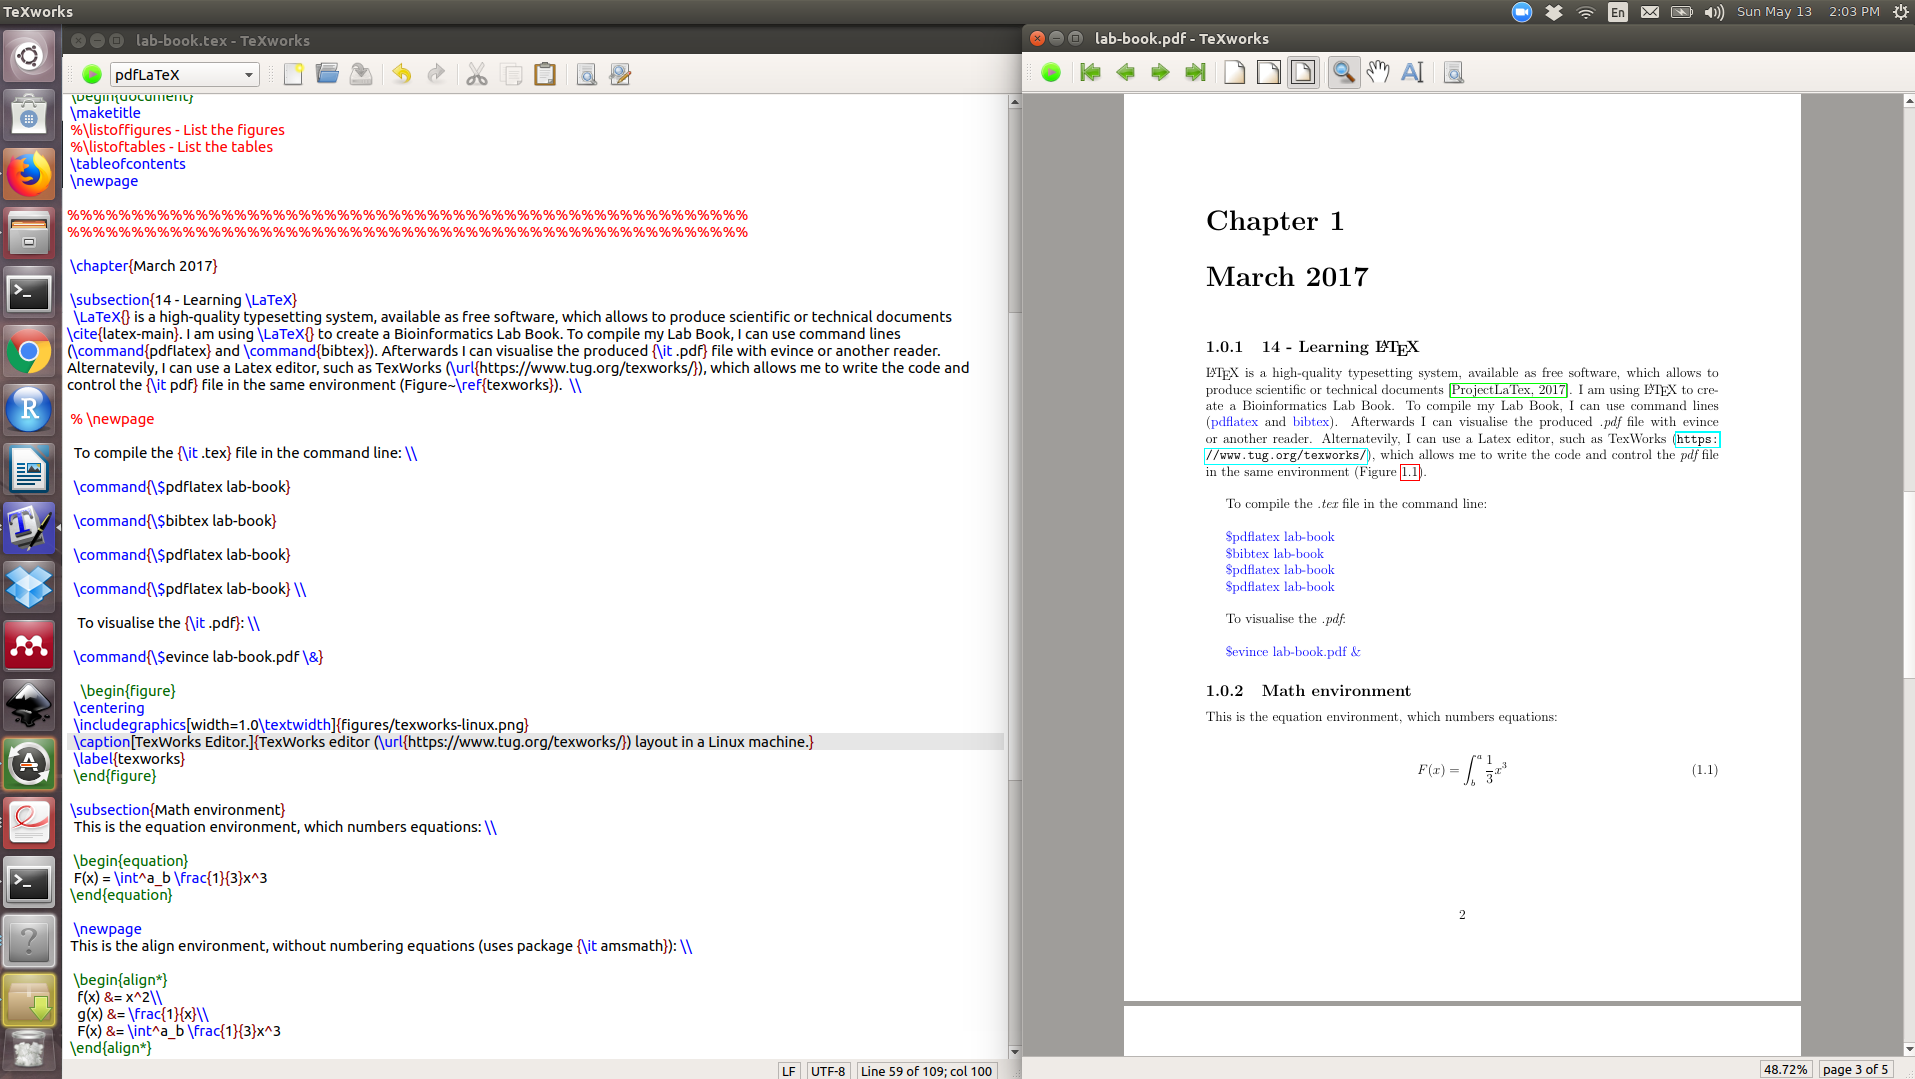
\includegraphics[width=1.0\textwidth]{figures/texworks-linux.png} 
  \caption[TexWorks Editor.]{TexWorks editor (\url{https://www.tug.org/texworks/}) layout in a Linux machine.}
  \label{texworks} 
  \end{figure}
  
 \subsection{Math environment}
  This is the equation environment, which numbers equations: \\
  
  \begin{equation}
  F(x) = \int^a_b \frac{1}{3}x^3
 \end{equation}
 
  \newpage
 This is the align environment, without numbering equations (uses package {\it amsmath}): \\
 
  \begin{align*}
   f(x) &= x^2\\
   g(x) &= \frac{1}{x}\\
   F(x) &= \int^a_b \frac{1}{3}x^3
 \end{align*}
 
  \subsection{15 - Short-term project proposal}
 Some text here. Incluing and referencing a table (table~\ref{table1}).
 
 \begin{itemize}
\item First numbered list item
\item Second numbered list item
\end{itemize}

\begin{table}[!htb]
  \caption{table0}
  \centering
  \begin{tabular}{ccc}
  \hline 
       species&changes&score \\
  \hline
       Macaque&4&0.0 \\
       Human&2&14.9 \\
       Orangutan&0&0.0 \\
       Pan&0&0.0 \\
       Gorilla&0&0.0 \\
  \hline
  \end{tabular}
  \label{table1}
 \end{table}

\chapter{Creation of data base of metagenomes and genomes}
\section{28}
\subsection{Bibliographic search for genomes}
Found a new possibility of phyla list. Because of this, there are four possibilities of list of microorganisms phyla, one of them, the SILVA database, is based in RNA sequences:
\begin{itemize}
\item The list of Prokariotic names with stading nomenclature \url{http://www.bacterio.net/-classifphyla.html}
\item SILVA database LSU(large subunit of ribosome) \url{https://www.arb-silva.de/browser/lsu/}
\item SILVA database SSU(small subunit of ribosome) \url{https://www.arb-silva.de/browser/ssu/}
\item PATRIC GENOMES \url{https://www.patricbrc.org/view/Taxonomy/2#view_tab=taxontree}
 \end{itemize}

The list of articles used until now is:
\begin{itemize}
\item 10.1038/nature14486
\item 10.1038/ismej.2013.111
\item 10.1038/ismej.2013.174
\item 10.1038/ismej.2016.43
\item 10.1038/nature12352
\item 10.1038/nature14486
\item 10.1038/nature21031
\item 10.1038/ismej.2015.233
\item 10.1038/ncomms13219
\item 10.1073/pnas.0801980105
\item 10.1111/1462-2920.13362
\item 10.1126/science.1132690
\item 10.1186/s40168-015-0077-6
\end{itemize}

\clearpage
\newpage
The list os correspondent phyla and articles is above:\\

\begin{center}
\begin{longtable}{ccc}
\caption{table 1}\\
\hline
  DOI&Phylum\\
\hline
10.1038/nature14486	&	Candidatus Falkowbacteria	\\
10.1038/nature14486	&	Candidatus Kuenenbacteria	\\
10.1038/nature14486	&	Candidatus Magasanikbacteria	\\
10.1038/nature14486	&	Candidatus Uhrbacteria	\\
10.1038/nature14486	&	Candidatus Moranbacteria	\\
10.1038/nature14486	&	Candidatus Azambacteria	\\
10.1038/nature14486	&	Candidatus Yanofskybacteria	\\
10.1038/nature14486	&	Candidatus Jorgensenbacteria	\\
10.1038/nature14486	&	Candidatus Wolfebacteria	\\
10.1038/nature14486	&	Candidatus Giovannonibacteria	\\
10.1038/nature14486	&	Candidatus Nomurabacteria	\\
10.1038/nature14486	&	Candidatus Campbellbacteria	\\
10.1038/nature14486	&	Candidatus Adlerbacteria	\\
10.1038/nature14486	&	Candidatus Kaiserbacteria	\\
10.1038/nature14486	&	C. S. yataiensis	\\
10.1038/nature14486	&	Pacebacteria	\\
10.1038/nature14486	&	Candidatus Collierbacteria	\\
10.1038/nature14486	&	Candidatus Beckwithbacteria	\\
10.1038/nature14486	&	Candidatus Roizmanbacteria	\\
10.1038/nature14486	&	Candidatus Saphirobacteria	\\
10.1038/nature14486	&	Candidatus Amesbacteria	\\
10.1038/nature14486	&	Candidatus Woesebacteria	\\
10.1038/nature14486	&	Candidatus Gottesmanbacteria	\\
10.1038/nature14486	&	Candidatus Levybacteria	\\
10.1038/nature14486	&	Candidatus Daviesbacteria	\\
10.1038/nature14486	&	Candidatus Curtissbacteria	\\
10.1038/nature14486	&	WWE3	\\
10.1038/nature14486	&	CPR3	\\
10.1038/nature14486	&	WS6	\\
10.1038/nature14486	&	Candidatus Berkelbacteria	\\
10.1038/nature14486	&	Candidatus Peregrinibacteria	\\
10.1038/nature14486	&	Candidatus Gracilibacteria	\\
10.1038/nature14486	&	CPR2	\\
10.1038/nature14486	&	Kazan	\\
10.1038/nature14486	&	Saccharibacteria (TM7)	\\
10.1038/nature14486	&	SR1	\\
10.1038/ncomms13219	&	Candidatus Kerfeldbacteria 	\\
10.1038/ncomms13219	&	Candidatus Komeilibacteria	\\
10.1038/ncomms13219	&	Candidatus Andersenbacteria 	\\
10.1038/ncomms13219	&	Candidatus Ryanbacteria	\\
10.1038/ncomms13219	&	Candidatus Niyogibacteria 	\\
10.1038/ncomms13219	&	Candidatus Tagabacteria 	\\
10.1038/ncomms13219	&	Candidatus Terrybacteria 	\\
10.1038/ncomms13219	&	Candidatus Vogelbacteria	\\
10.1038/ncomms13219	&	Candidatus Zambryskibacteria 	\\
10.1038/ncomms13219	&	Candidatus Taylorbacteria	\\
10.1038/ncomms13219	&	Candidatus Sungbacteria	\\
10.1038/ncomms13219	&	Candidatus Brennerbacteria 	\\
10.1038/ncomms13219	&	Candidatus Spechtbacteria 	\\
10.1038/ncomms13219	&	Candidatus Staskawiczbacteria 	\\
10.1038/ncomms13219	&	Candidatus Wildermuthbacteria	\\
10.1038/ncomms13219	&	Candidatus Portnoybacteria 	\\
10.1038/ncomms13219	&	 Candidatus Woykebacteria 	\\
10.1038/ncomms13219	&	Candidatus Blackburnbacteria 	\\
10.1038/ncomms13219	&	Candidatus Chisholmbacteria 	\\
10.1038/ncomms13219	&	Candidatus Buchananbacteria	\\
10.1038/ncomms13219	&	Candidatus Jacksonbacteria 	\\
10.1038/ncomms13219	&	Candidatus Veblenbacteria	\\
10.1038/ncomms13219	&	Candidatus Nealsonbacteria 	\\
10.1038/ncomms13219	&	Candidatus Colwellbacteria 	\\
10.1038/ncomms13219	&	Candidatus Liptonbacteria 	\\
10.1038/ncomms13219	&	Candidatus Harrisonbacteria 	\\
10.1038/ncomms13219	&	Candidatus Yonathbacteria 	\\
10.1038/ncomms13219	&	Candidatus Lloydbacteria	\\
10.1038/ncomms13219	&	Candidatus Abawacabacteria	\\
10.1038/ncomms13219	&	Candidatus Doudnabacteria	\\
10.1038/ismej.2013.111	&	Candidatus Poribacteria	\\
10.1111/1462-2920.13362	&	Candidatus Desantisbacteria	\\
10.1038/nature12352	&	Candidatus Omnitrophica	\\
10.1038/nature12352	&	Candidatus Aminicenantes	\\
10.1126/science.1132690	&	Candidatus Micrarchaeota	\\
10.1038/nature14486	&	Candidatus Magasanikbacteria	\\
10.1073/pnas.0801980105	&	Candidatus Korarchaeota	\\
10.1038/nature12352	&	Candidatus Fervidibacteria	\\
10.1038/nature12352	&	Candidatus Aenigmarchaeota	\\
10.1038/ismej.2016.43	&	Candidatus Fermentibacteria	\\
10.1038/ismej.2013.174	&	Candidatus Bathyarchaeota	\\
10.1016/j.cub.2015.01.014	&	Candidatus Woesearchaeota	\\
10.1016/j.cub.2015.01.014	&	Candidatus Kryptonia	\\
10.1038/nature12352	&	Candidatus Diapherotrites	\\
10.1038/nature12352	&	Candidatus Latescibacteria	\\
10.1038/nature21031 10.1038/ismej.2015.233	&	Candidatus Thorarchaeota	\\
10.1038/ncomms13219	&	Candidatus Lindowbacteria	\\
10.1038/nature12352	&	Candidatus Parvarchaeota	\\
10.1038/nature12352	&	Candidatus Cloacimonetes	\\
10.1038/nature12352	&	Candidatus Hydrogenedentes	\\
10.1038/nature12352	&	Candidatus Acetothermia	\\
10.1038/nature12352	&	Candidatus Nanohaloarchaeota	\\
10.1038/ncomms13219	&	Candidatus Eisenbacteria	\\
10.1186/s40168-015-0077-6	&	candidate division WOR-3	\\
 \hline
  \end{longtable}
\end{center}

\section{28}

\subsection{Bibliographic search for metagenomes}
The reserarch for coral metagenomes started last year. The actual list is:
\begin{longtable}
mgm4440319.3	\\
mgm4440370.3	\\
mgm4440371.3	\\
mgm4440372.3	\\
mgm4440373.3	\\
mgm4440374.3	\\
mgm4440375.3	\\
mgm4440376.3	\\
mgm4440377.3	\\
mgm4440378.3	\\
mgm4440379.3	\\
mgm4440380.3	\\
mgm4440381.3	\\
mgm4445755.3	\\
mgm4445756.3	\\
mgm4480739.3	\\
mgm4480740.3	\\
mgm4480741.3	\\
mgm4480748.3	\\
mgm4480750.3	\\
mgm4487909.3	\\
mgm4487910.3	\\
mgm4487911.3	\\
mgm4516541.3	\\
mgm4516694.3	\\
mgm4653307.3	\\
mgm4694757.3	\\
mgm4694758.3	\\
mgm4694759.3	\\
mgm4694760.3	\\
SRR1275409	\\
SRR1275449	\\
SRR1283349	\\
SRR1283371	\\
SRR1283377	\\
SRR1283433	\\
SRR1283435	\\
SRR1283437	\\
SRR1286223	\\
SRR1286225	\\
SRR1286226	\\
SRR1286227	\\
SRR1286229	\\
SRR1286232	\\
SRR1822488	\\
SRR1822516	\\
SRR3499156	\\
SRR3569370	\\
SRR3694369	\\
SRR3694370	\\
SRR3694371	\\
SRR3694372	\\
SRR5215424	\\
SRR5215454	\\
SRR5215455	\\
SRR5215456	\\
SRR5215457	\\
SRR5215458	\\
SRR5215462	\\
SRR5605611	\\
\end{longtable}

I found these metagenomes in the article: "Metagenomic analysis reveals a green sulfur bacterium as a potential coral symbiont"
SRR2937345
SRR2937346
SRR2937347
SRR2937348
SRR2937349
SRR2937350
SRR2937351
SRR2937352
SRR2937353
SRR2937354
SRR2937355
SRR2937356
Espécie: Platygyra carnosa
Healthy

I uptated the file pmc_results_1.txt in the repository Lab_book

 \bibliographystyle{apalike}
 \bibliography{ref}



 \end{document}
